\biohead{Hugh Croskery}{}

\begin{figure}
 \centering
 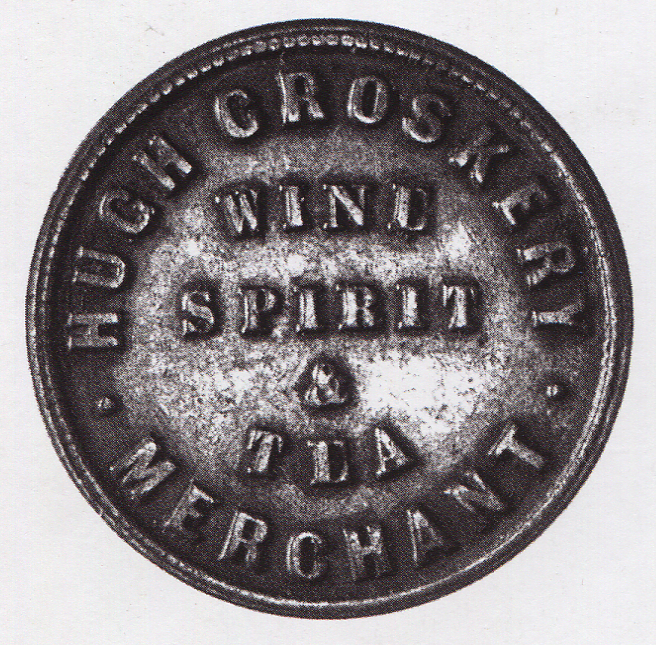
\includegraphics{photos/Hugh_Croskery_token}
 \caption{A `token' from Hugh Croskery's grocery shop.\cite{DownTown2}}
\end{figure}

Hugh Croskery was born in 1803, in Downpatrick, County Down, Northern Ireland (his parents are not known).

He married \bioref{Charlotte_Wallace_Brown} on 9 May 1834 at the First Presbyterian Church, in Ballynahinch, County Down and they had eight children:  Hugh Croskery (1835--1886), Ann Croskery (1836--1931), Alexander Brown Croskery (1838--1897), Albert James Croskery (1840--1865), Horatio Collingwood Croskery (1842--1929), Frederick C. Croskery (1845--?),  Captain \bioref{Samuel_Maxwell_West_Croskery} and Wallace Brown Croskery (1851--1926). 

His occupation was as a Grocer, wine, spirit and general merchant, in 1846 living in Scotch Street, Downpatrick and then in Market Street in 1850. An advertisement in the Downpatrick Recorder on 30 November 1847 read:
``Wanted: an Apprentice to the Spirit and Grocery Business. Apply to the Subscriber, Hugh Croskery.''\cite{HCroskeryAdvert}  He was also a publican in Scotch Street \cite{HughCroskeryOccupation}. By 1874 his occupation was noted as being a retired Ship owner, and he was also a mine owner and farmer. 

He died after 1897: at the time he was living in Dublin (as mentioned in a letter dated 1897 from his son West to his daughter-in-law Minnie, after his son Alexander had died in New Zealand (see page \pageref{Samuel_Maxwell_West_Croskery}). \cite{HughCroskeryDeath}.
